\section{Application 2: Sampling from Covariance Matrices (e.g. for BayesOpt)}

\gp{todo}

\begin{figure}[t!]
  \centering
  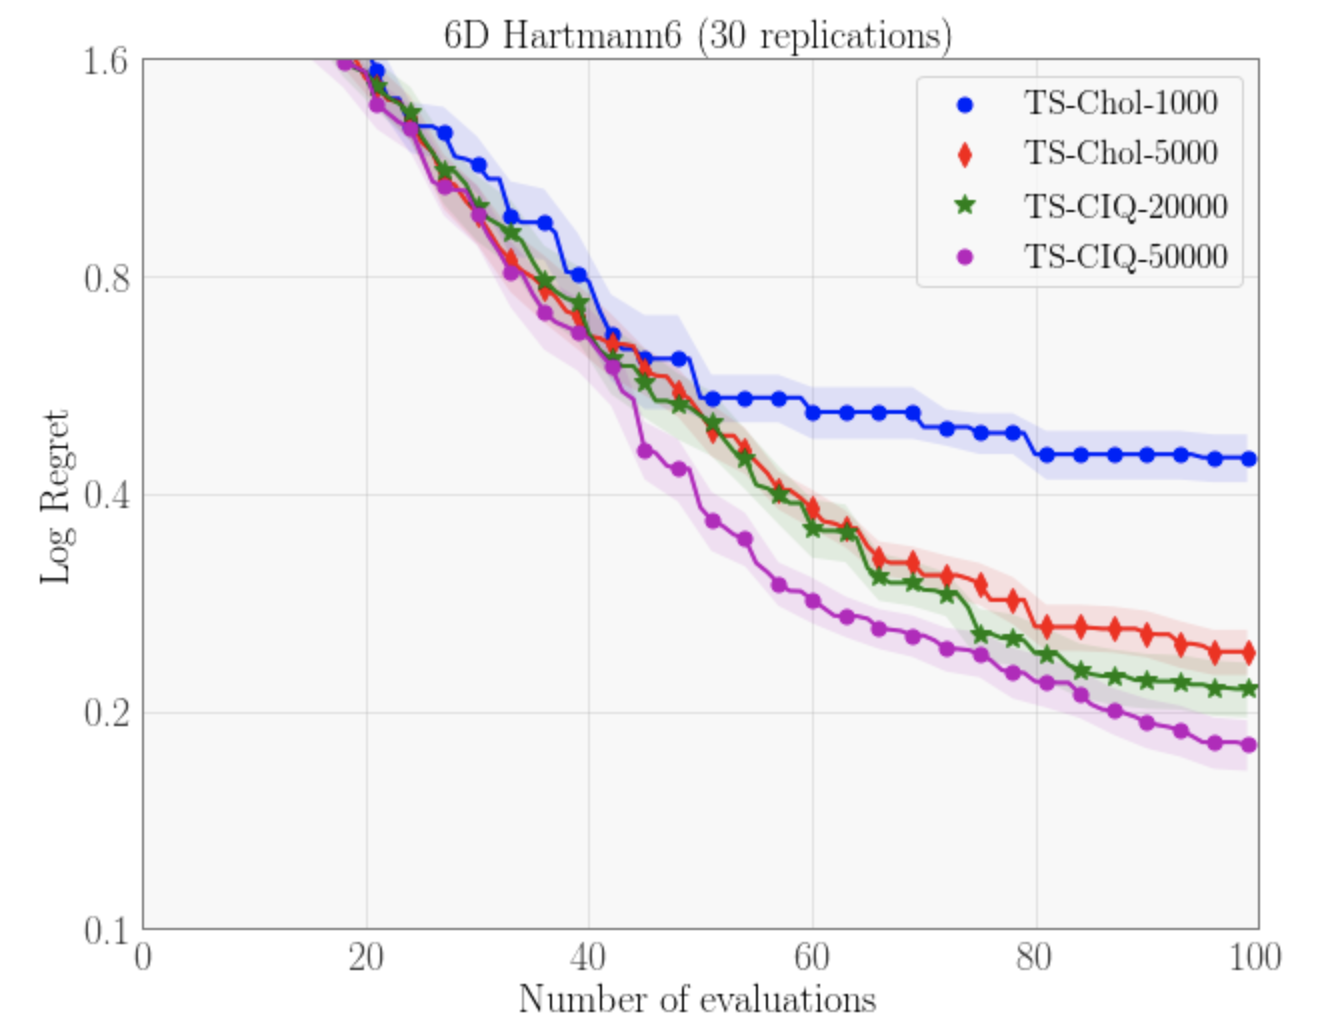
\includegraphics[width=0.72\linewidth]{figures/hartmann6.png}
  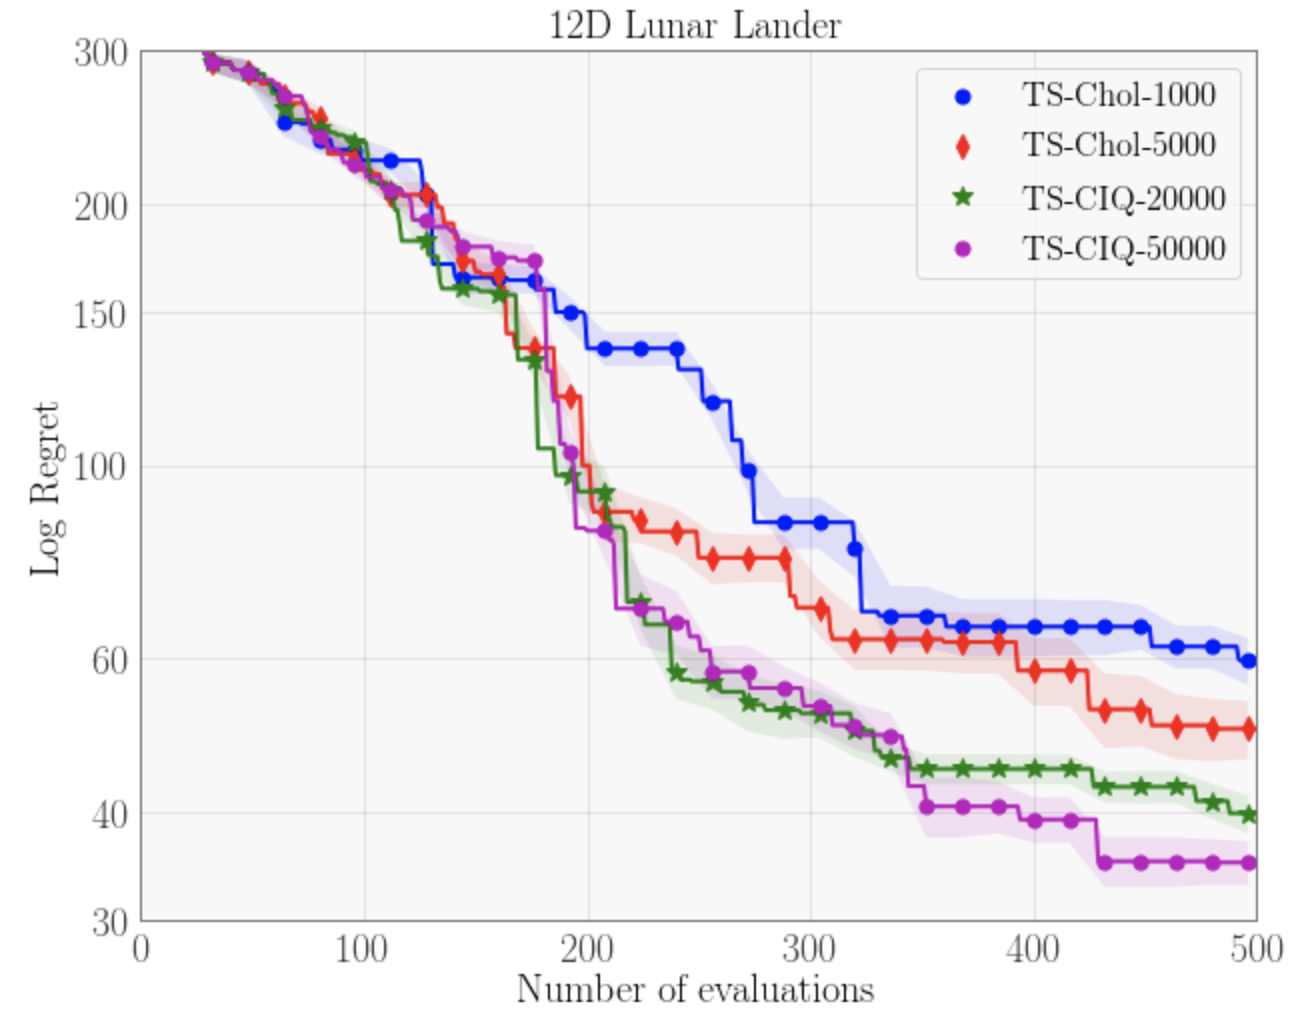
\includegraphics[width=0.7\linewidth]{figures/lunar_lander.png}
  \caption[
    A comparison of sampling methods for Bayesian optimzation (BayesOpt) via Thompson sampling.
    BayesOpt is applied to the Hartmann ($D=6$) and Lunar Lander ($D=12$) functions.
  ]{
    A comparison of sampling methods for Bayesian optimzation (BayesOpt) via Thompson sampling.
    BayesOpt is applied to the ({\bf top}) Hartmann ($D=6$) and ({\bf bottom}) Lunar Lander ($D=12$) functions.
    Methods: TS-Chol-$\langle T \rangle$ draws posterior samples with Cholesky at $T$ candidate points.
    TS-CIQ-$\langle T \rangle$ draws posterior samples with CIQ.
    Larger $T$ (number of candidate point) results in better optimization.
    CIQ enables scaling to $T\geq50,\!000$.
  }
  \label{fig:hartmann6}
\end{figure}

\begin{figure}[t!]
  \centering
  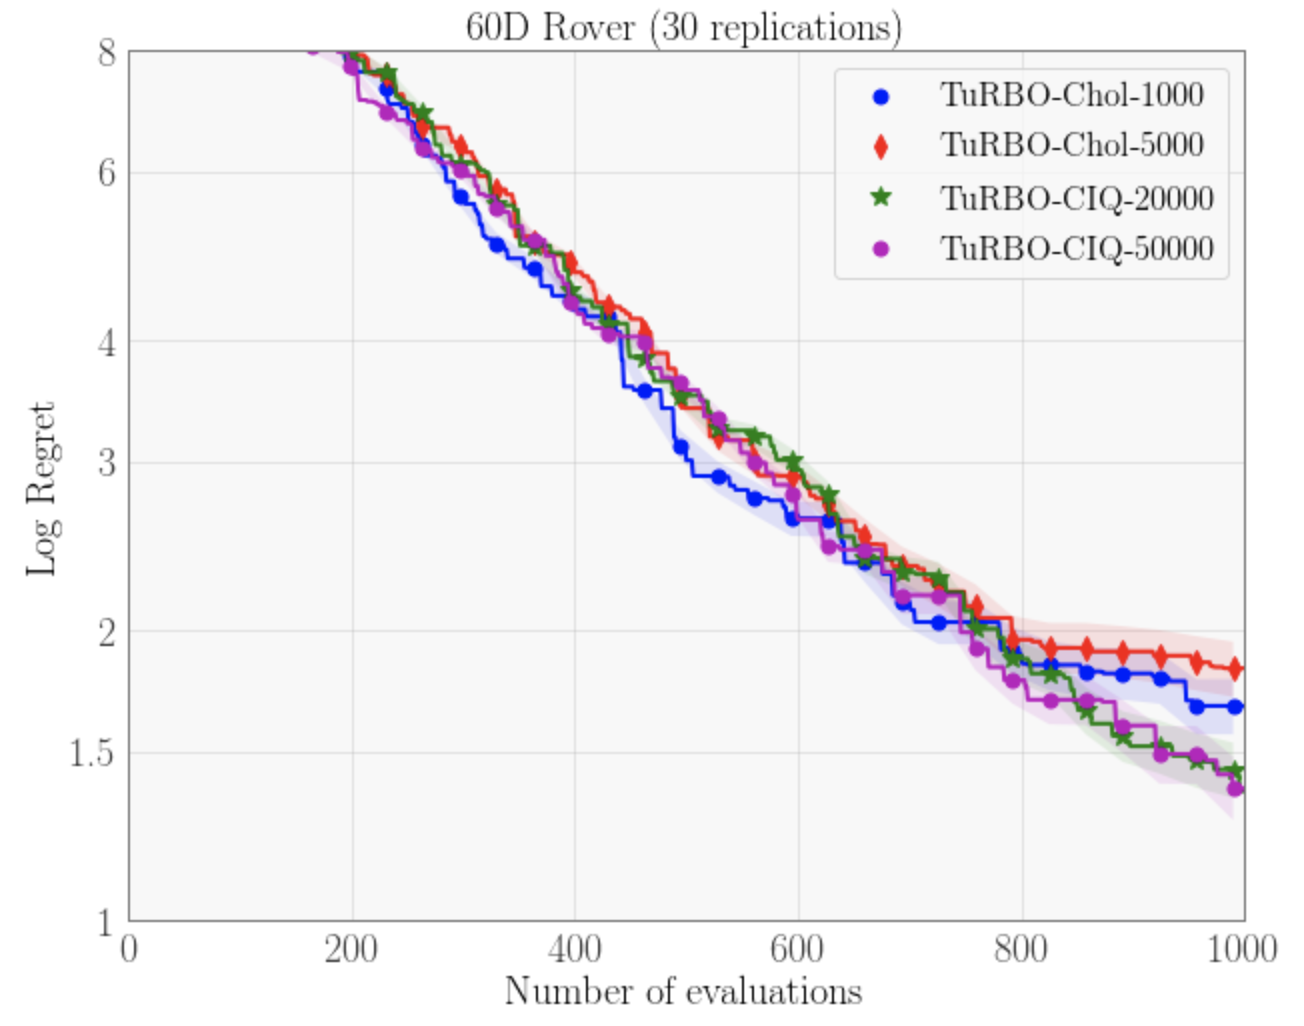
\includegraphics[width=0.7\linewidth]{figures/rover.png}
  \caption[
    A comparison of sampling methods for Bayesian optimzation (BayesOpt) via TuRBO \cite{eriksson2019scalable}.
    BayesOpt is applied to the Rover ($D=60$) function.
  ]{
    A comparison of sampling methods for Bayesian optimzation (BayesOpt) via TuRBO \cite{eriksson2019scalable}.
    BayesOpt is applied to the Rover ($D=60$) function.
    Larger $T$ (number of candidate point) results in better optimization.
    CIQ enables scaling to $T\geq50,\!000$, whereas Cholesky is limited to $T\leq5,\!000$
  }
  \label{fig:hartmann6}
\end{figure}
